% Identification of safety critical system components?
% Definition of simulation requirements & constraints
% Gamification strategy: what should the objective be, how should the user be engaged -> use the definition of Game to point this out
% Conceptual Design of Game Engine (Architecture & Features)
% Conceptual design of scenes / characters / challenges (goals, visual elements, structure)
% validation method used

\chapter{Conceptualization}\label{ch:design}
The conceptualization chapter focuses on the definition of requirements regarding both the game engine and the game implementation, such as
general approach to the framework and features required.
The major goals that should be achieved by the player are set, as well as the basic game play, rules and appearance of the games' environment is described.
Furthermore, an overview of components that should be developed and designed for the game is given by using generic layouts for different scenes
and functions of the game.
A basic concept for level design is developed.

\section{Requirements}\label{sec:requirements}
As the major objective of the game is to create a fun environment for users to test and familiarize themselves with the topic of
aircraft system design and different architectures used, the game requirements need to be defined.
\\
The game is designed to acquaint players with the notions of redundancy and system failures, including various
failure categories such as common-mode and common-cause failures.
While offering a blend of enjoyment and interaction, the game's primary objective should not be solely amusement but
rather a combination of entertainment and education.
In this context, education aims to spark interest in the relatively unfamiliar subject of aircraft systems.
\\
The game should be accessible to players without any prior knowledge of the subject matter and easy to engage with.
Supplementary explanations and details can be provided but should not be essential for comprehending the core gameplay.
The game should be suitable for open-door events and must accommodate gamepad integration, as playing with a mouse and
keyboard may not be as enjoyable in such settings.

\section{Genre}\label{sec:genre}
Genres that were considered going into the game development process were \textit{Simulation}, \textit{Puzzle}, \textit{Platform} and \textit{Serious}.
Eventually it was decided that the game is going to be designed as a serious puzzle game with simulation elements, where the user has different elements to build a system from.
As the game is supposed to attract interest about the topic of aircraft systems.
Puzzle games offer a way for the player to logically or conceptually solve levels, which is usually realized without
implementing any sort of time pressure~\cite{10.5555/2544002}.
That is also going to be the case in this game, however some score mechanics and different calculations may be implemented to reflect
the rating of the player.
\section{Finding a name}\label{sec:finding-a-name}
The process of finding a name was guided by trying to represent aircraft, system engineering and the puzzling aspect of the game.
A list of different names was proposed, that combine some or all of the former-mentioned elements.
The following names were available for further selection and refinement.
\begin{itemize}
    \item SkyLogic
    \item AeroSystems Architect
    \item Am I an Aircraft Systems Engineer?
    \item Aircraft Systems Engineering Puzzle
    \item Aircraft Systems Architect
\end{itemize}
The final name that was chosen for the game in order to design a logo and icon is \textit{Aircraft Systems Architect}.
Figures~\ref{fig:logo} and~\ref{fig:logo-icon} show the games' logo and icon designs.
\begin{figure}
    \centering
    
\includegraphics[width=0.7\textwidth]{Pictures/res/concept/aircraft-systems-architect-logo}
    \caption{Game logo}
    \label{fig:logo}
\end{figure}
\begin{figure}
    \centering
    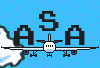
\includegraphics[width=0.7\textwidth]{Pictures/res/concept/asa-logo}
    \caption{Game logo icon}
    \label{fig:logo-icon}
\end{figure}

\section{Game Engine Design}\label{sec:game-engine-design}
In this section, an overview of the game engine architecture and core features is given.
The design principles and development methodologies are clarified and challenges regarding the implementation will be defined.

\subsection{Architecture}\label{subsec:architecture}
The game engine uses an entity component system approach, which aims to decompose the game objects (entities) into small, reusable and interchangeable
components, that act as simple data containers to define properties of an object.
The game engine follows an object-oriented programming approach, where entities and components are designed to be easily extendable and inheritable.
This allows for an easy creation of new types of entities or components by reusing and extending existing ones, without modifying the core engine code.
To achieve this, a set of base classes for entities, components and systems is defined, which can be subclassed and implemented to provide the custom data and
properties and logics needed.
Components should simply act as data containers, which also follows the data encapsulation approach typically used in object-oriented programming, as
the interface to access the data within a component is provided by the components' getter and setter methods.
\\
The game engine follows a modular approach, where a set of systems - which is either pre-defined by the core game engine (e.g.\ rendering, sounds) or
a custom implementation by the game - is executed by a game loop to handle inputs, game logics and updates to the entities and components.
This modular approach allows for an easy addition or removal of systems depending on the game implementation, without affecting the game loop.
It also enables for optimizations such as parallelization of the execution of the systems, which leads to performance and scalability improvements.
However, in the scope of this thesis, it may not be necessary to parallelize the game systems.

\subsection{Features}\label{subsec:features}
The core features provided by the game engine are rendering, audio handling, input handling, resource management and language management.
\\
The rendering system provides handling of different screen dimensions, options for fullscreen visualization and window mode, and allows
for rendering of different graphical objects, such as text, shapes, images or animations.
Rendering is done solely in 2D.
The rendering system also provides a scaling engine, which is used to correctly detect the actual screen position against the design point and scale it accordingly
(e.g.\ a game may be developed for 1920x1080px screens, but can also be used on other screen sizes).
\\
\\
The audio system enables the game engine to play and mix different types of sounds and music with a support for different audio formats and codecs.
It is able to handle looped audios and helps in creating and enhancing the game environment.
\\
\\
The game engine provides a flexible input system that allows to capture a variety of user inputs, including keyboards, mouse and gamepad events.
The input system supports a customization of different key bindings to functions, as it serves as a queue of events happening during the game which
may then be processed by other systems.
Events are queued by recording the inputs of every input device, e.g.\ a state change of a button or key.
\\
\\
Resource management is a built-in feature of the game which enables the developer to easily load different file types, such as images or XML files.
This includes languages, tile sets, high score files and level files of a pre-defined format.
The resource manager may be replaced with a custom resource loader, depending on the games' needs and requirements.
\\
\\
The game employs a language management system that uses IDs (tags) instead of actual text for each text string.
A processor parses all available language files in XML format and generates a look-up table that associates each ID with its corresponding text string.
In the Rendering Engine, text is displayed in the language currently selected for the game.
This approach allows for multi-language support without the need for modifying game code.
Language files can be translated and simply incorporated into the game, enabling users to switch languages as desired.
\section{Game Environment Design}\label{sec:game-environment-design}
Before implementing the game itself, a concept and idea for the game is developed and a prototype is built, which is refined during the
actual implementation process of the game.
In this chapter, the process of conceptualizing and designing the game, including mechanics and gameplay, graphic concepts and
level design is explained.

\subsection{Intended Gameplay}\label{subsec:intended-gameplay}
The player is playing an aircraft mechanic, who is supposed to investigate systems for possible failures and improve the given systems or
build new systems according to given requirements.
The player is given instructions by an aircraft engineer and a tablet device with some applications to show necessary
information, requirements and tips.
There are multiple levels with advancing difficulty that may be played.
Each of these levels shows and conveys different concepts used in system engineering.
To solve the puzzle levels, the user has different components to choose from in the inventory (also called the build panel), that
can be added to the current system configuration by drag and drop.
Components can be connected by using cables and putting them in the correct places and rotations.
As the game is grid-based, there are limited possibilities of component placement, which have to be considered in level design, however most levels
may be solved in different ways, which are to some degree more or less efficient.
This is represented by the score that is calculated at the end of each level after validating the systems correct functionality, which gives
a hint to the player where he or she may perform better in order to score higher.
\\
The detailed game mechanics are described in the next section~\ref{subsec:game-mechanics}.

\subsection{Game Mechanics}\label{subsec:game-mechanics}
As the general intended game play was already stated in the previous chapter, the detailed game mechanics are going to be described in this section.
\\
In each level, a defined set of components is already available on the game grid, which may or may not be replaceable, depending on the given
information contained in the level file.
\\
Each component has defined simulation parameters such as failure probability, failure detection rate and requirements to the amount of
maximum out-of-control states and minimum correct states, which can not be changed by the user.
Another set of components is added to the users build panel in each level, where they can be placed by drag and drop to the game grid.
The goal is to use the given space on the grid efficiently and build a system that has a failure ratio below the requirement which is defined as a level goal.
Components can be connected by using different cables (red, blue, green, yellow), which simply represent different layers of cables, so multiple
cables can be placed on a single grid tile.
Cables can be rotated to correctly connect components or cables of the same type.
Each cable port type color is also shown on the component itself to make clear, which components have in- and outgoing cable ports
that cables may be connected to.
\\
After setting up the system configuration, the player can start a simulation.
This simulation calculates the markov chain of the given system and adds up the failure probability of all states that lead to a system failure with the given
input requirements.
\\
Comparing this result to the goal leads to a passed or failed level, while the distance from the players' system to the target also matters when it comes to calculating
the score, which consists of exactly this distance, the remaining components in the players inventory and a base score for each level.
During the simulation process, the aircraft starts flying through the sky to give a visualization that something is happening, as with increasing
level size the time to calculate the probabilities rises accordingly, as stated in section~\ref{subsec:markov-process}.
\\
If the level is passed successfully, a visualization of that is given by showing a score board and fireworks, if the level is failed, the aircraft
shows explosions instead.

\subsection{Graphic Design}\label{subsec:graphic-design}
The objective of the graphic design process was to envision the overall layout of the game environment and establish the
appearance and style of the primary components involved.
Throughout this process, placeholders were employed in a prototype game to illustrate the positioning of various UI and game elements.
The graphic design process was iterative, with most graphics undergoing numerous revisions during the game development.
\\
Owing to the need to maintain simplicity for the target audience, the graphic design was also kept clean and straightforward.
As a result, a classic 8-bit graphic style was adopted for all game visuals, including the UI. Additionally,
the retro aesthetic has been widely utilized in numerous games previously, which helps to emphasize the gamified approach more evidently.
A color palette consisting of predominantly bright colors and various shades of gray was applied across all graphics.
\\
The following figures show the general layout concept of the level
menu scene~\ref{fig:level-menu-scene-concept} and the game scene~\ref{fig:game-scene-concept}.
\begin{figure}
    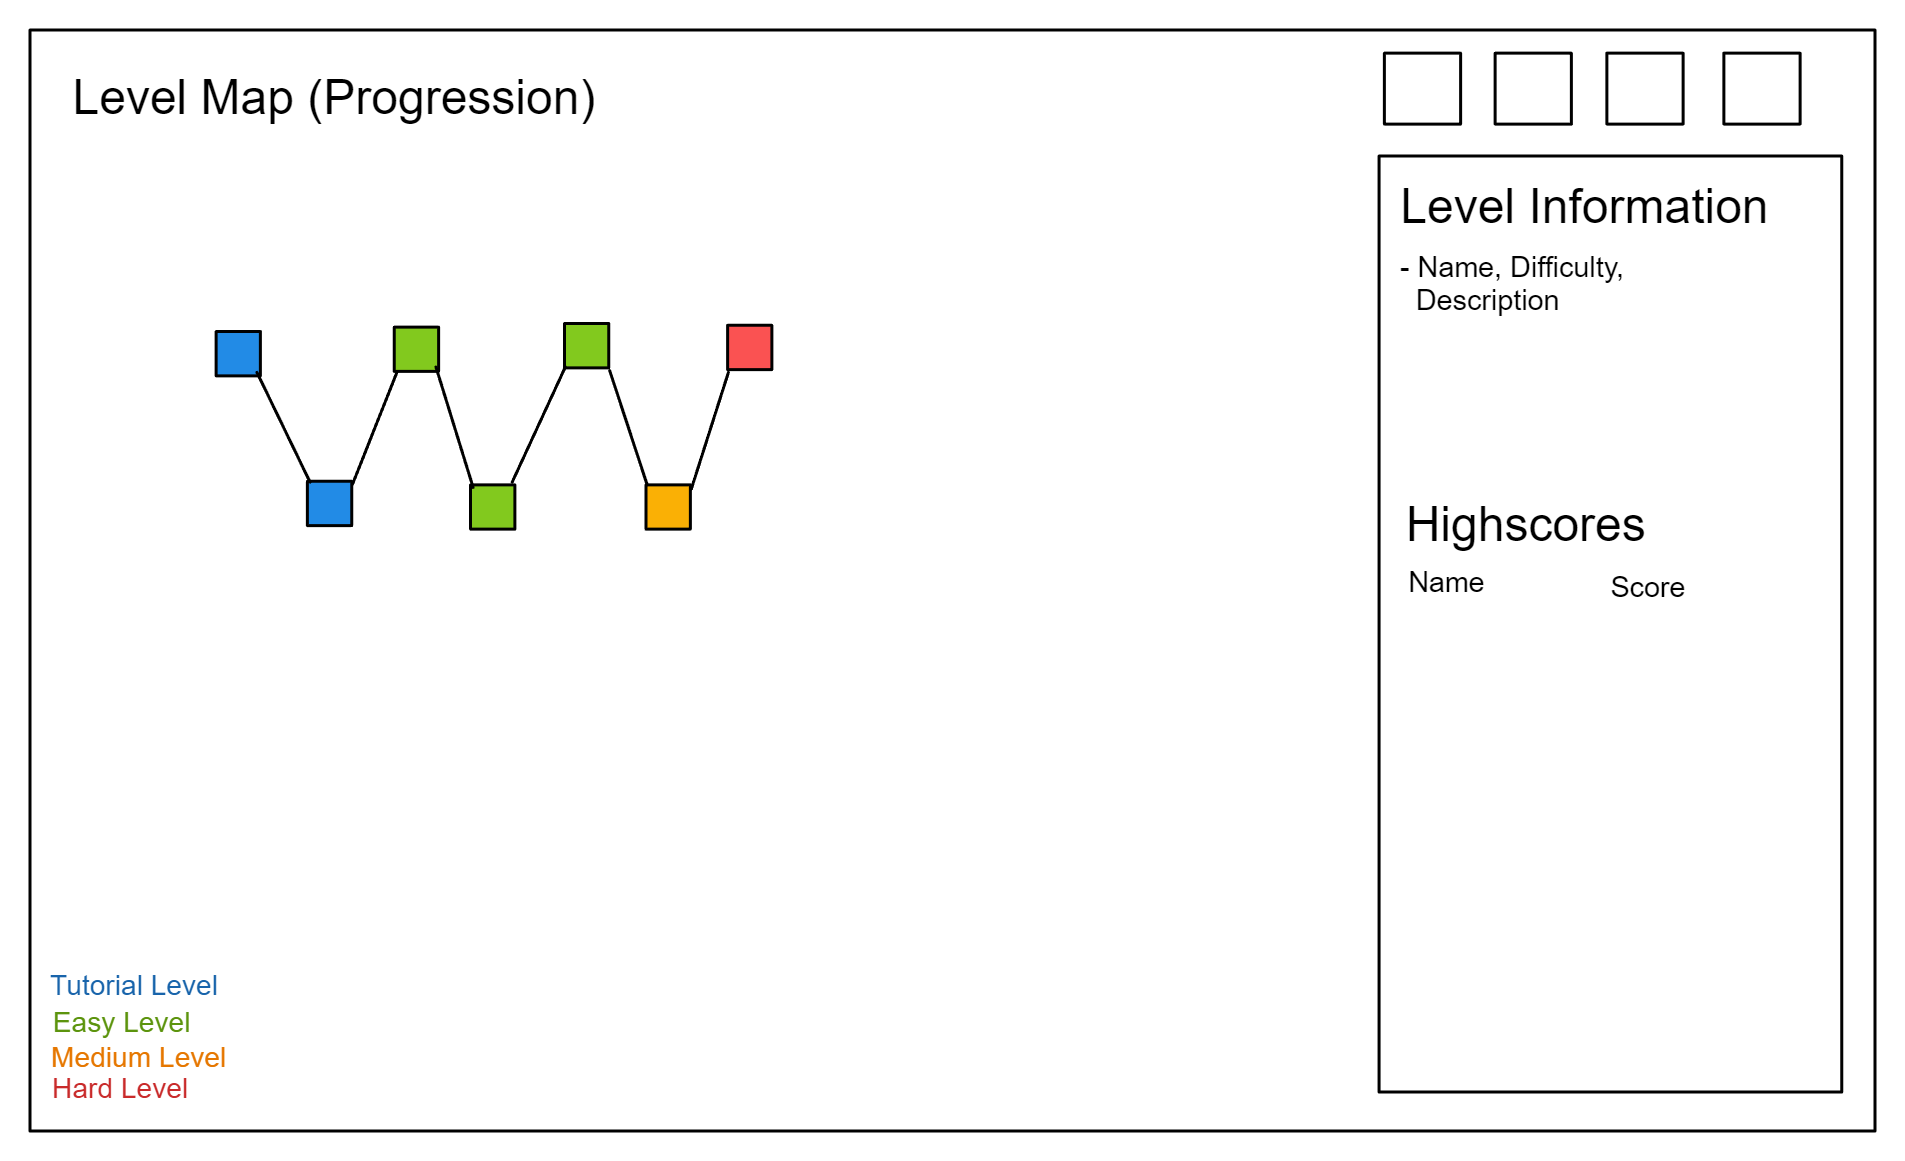
\includegraphics[width=0.75\textwidth]{Pictures/res/concept/level-menu-scene-concept}
    \caption{Level menu scene concept}
    \label{fig:level-menu-scene-concept}
\end{figure}
\begin{figure}
    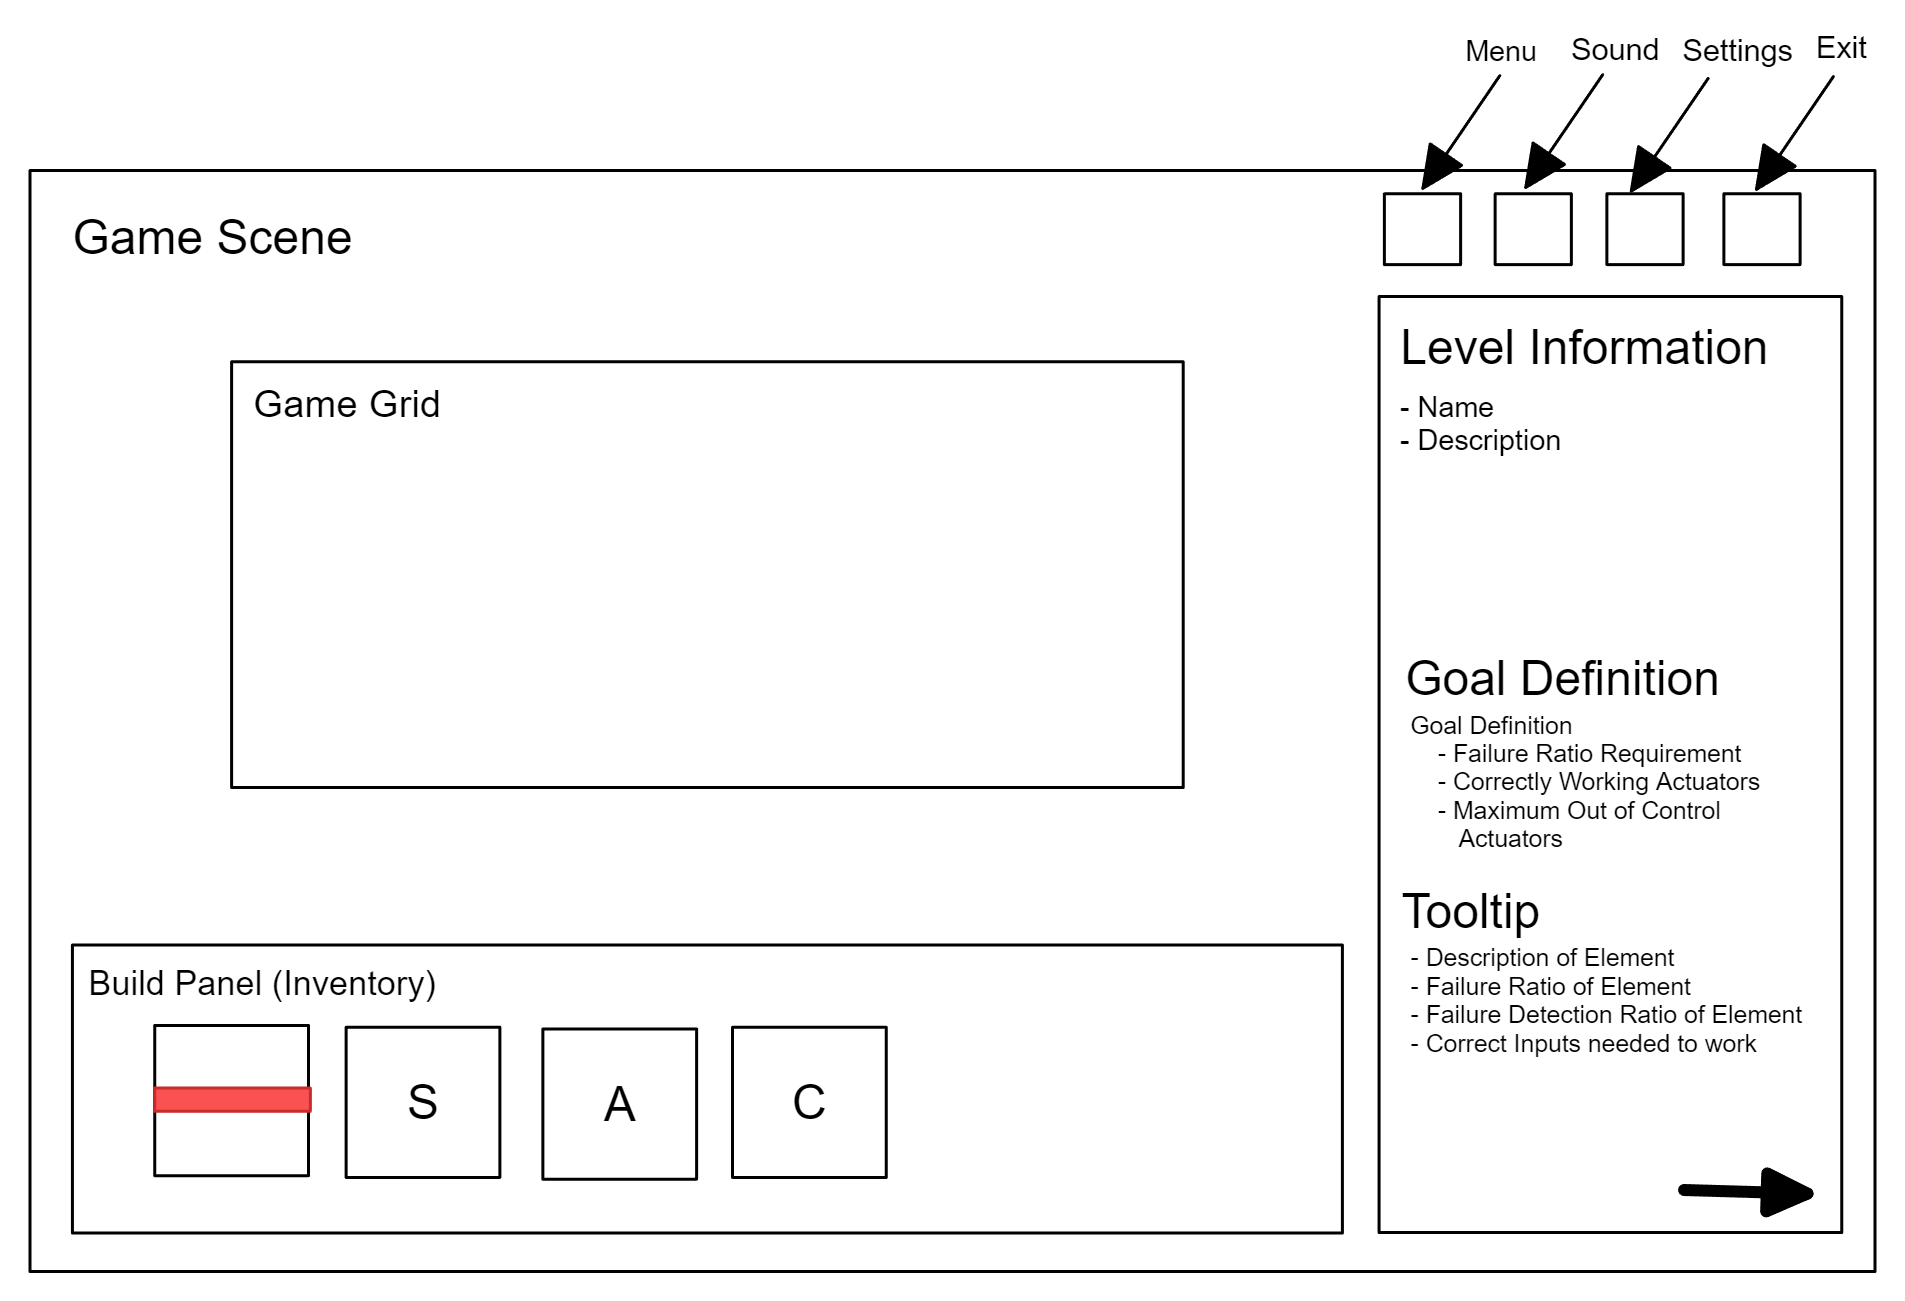
\includegraphics[width=0.75\textwidth]{Pictures/res/concept/game-scene-concept}
    \caption{Game scene concept}
    \label{fig:game-scene-concept}
\end{figure}
According to the concept scene layouts, the following components have to be designed:
\begin{itemize}
    \item Screen backgrounds
    \item Background tiles, placeholder tiles
    \item Simulation components: actuators, sensors, computers, cables, \ldots
    \item Build panel
    \item Information panel
\end{itemize}

\subsection{Sound Design}\label{subsec:sound-design}
To establish ambiance and deliver an 8-bit-inspired experience, the game will utilize open-source music.
Ideally, the music should be loopable and available under an open-source license.

\subsection{Level Design}\label{subsec:level-design}
The level design is a main part of this work, as the progression through the game and the process of explaining different concepts
within aircraft system design is heavily influenced by this.
Therefore, some levels were conceptualized before the implementation, to have a guideline for the actual implementation.
Levels are categorized in difficulties, ranging from tutorial to hard.
When passing a level, the user unlocks new levels to progress through the game, however the progression may be turned off and the user can choose from all
levels.
\\
Tutorials should guide the user through the features of this game and provide some insight on the basic gameplay and a general
understanding of aircraft systems, failures and redundancy concepts.
A visual representation of this is needed to provide enough input for younger age-groups to play and understand the game.
However, for other users, some more in-depth knowledge is also provided in order to better understand calculations, simulations and
game logic in the background.
Tutorial levels explain the basic usage, such as cable and component (re-)placement and the different safety requirement
categories.
\\
The categories are described by colors, from red (catastrophic) to blue (no safety effect).
Each component that can be built in the level also has this information to it, so the user can visually see a representation
of the criticality and the effect of the objects to the system and its requirements.
Each level goal is defined by a safety requirement and a minimum count of correctly operating actuators (or other components, such
as flight control computers, sensors, \ldots).
As the user progresses through the levels, there will be harder goals in safety requirements that need to be solved by using
redundancy concepts or mechanisms such as voting.
As this work aims to explain most of the basic concepts, some levels should also take into consideration common-mode and common-cause
failures.
\\
The following levels have been conceptualized for this game by default:
\begin{enumerate}
    \item Tutorials to explain basic game concept and system engineering concepts
    \item Duplex Systems with and without cross-strapping
    \item Triplex Systems
    \item Systems with multiple actuators
    \item Systems with duplex sensors
    \item Common-Mode Failure scenario
    \item Common-Cause Failure scenario
\end{enumerate}
During the conceptualization, high-level designs for each level, including layouts, objectives and possible additional content were created.
Sketches and visualizations of the level ideas helped to create a baseline for the implementation that was used later during development of the levels.
During the implementation and production process of the game, most of the level designs were revised and adjustments were made, which is also
an iterative task where updates may be needed in the future.
\\
The finalized level designs and implementations will are shown in section~\ref{subsec:level-implementation}.
\\
Additionally, through a build mode the user is able to set up new levels including the requirements / level goal via the built-in
frontend, which then saves the level to a new xml file.

\subsection{Tutorials}\label{subsec:tutorials}
In order to effectively convey gameplay and concepts like redundancy, characters have been designed to engage in dialogue with the player,
making the experience more user-friendly and interactive despite the necessity of reading.
The game features two characters: one representing the player as an aircraft mechanic responsible for repairing
and examining various aircraft systems, and the other as an aircraft systems engineer who provides instructions and guidance throughout the game.
These characters appear during dialogues and tutorials to enhance player engagement.

\subsection{Language}\label{subsec:language}
As the game is supposed to be used by a broad audience, especially in Germany and at the University Day of the University of Stuttgart, there should be an option
to change the language.
Therefore, english, german and a simplified version of the german language file are supported by default.